% Number 640
% BFPM Tension KFriction
% Half Atwood - sliding at const. v
% JG

% Watermark
\AddToShipoutPicture*{\BackgroundPic}

\addtocounter {ProbNum} {1}

\begin{floatingfigure}[r]{.2\textwidth}
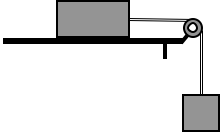
\includegraphics[scale=.6]{/Users/jgates/desktop/latex/pics/halfatwood3}
\end{floatingfigure}
 
{\bf \Large{\arabic{ProbNum}}} A 2 kg box sits on a rough (non-frictionless) table. It is connected by a massless string to a hanging 1 kg box.  If I give the box a short push to start it moving to the left, it will slide at a constant speed.
 
\bigskip
What is the coefficient of kinetic friction between the box and the table?\paragraph{}
\noindent
\vfill

%\hfill 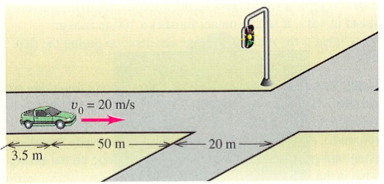
\includegraphics[scale=.85]{/Users/jgates/desktop/latex/pics/redlight.png}
\newpage
